\documentclass[fleqn]{jbook}
\usepackage{physpub}

\begin{document}

\begin{question}{$B@l96(B $BLdBj(B5}{}

$B8GBN7k>=Fb$NEE;R$K$D$$$F<!$NLd$KEz$($h!#(B
\begin{subquestions}
\SubQuestion
  $B7k>=Fb$G<~4|E*$KJQ2=$9$k%]%F%s%7%c%k>l(B$U(\vec{r})$$B$NCf$r1?F0$9$k(B
  $BEE;R$KBP$9$k%7%e%l!<%G%#%s%,!<J}Dx<0(B
%
  \[ H\Psi=\left(-\frac{\hbar^2}{2m}\vec{\nabla}^2+U(\vec{r})\right)
     \Psi=E\Psi,\hspace{1cm} U(\vec{r}+\vec{R})=U(\vec{r}) \]
%
  $B$N8GM-4X?t(B$\Psi(\vec{r})$$B$O!"(B$\vec{k}$$B$rGH?t%Y%/%H%k$H$9$k$H$-(B
%
  \begin{equation}
    \Psi(\vec{r}+\vec{R})=e^{i\vec{k}\vec{R}}\Psi(\vec{r}) \eqname{1}
  \end{equation}
%
  $B$H$$$&@-<A(B($B%V%m%C%[$NDjM}(B)$B$r;}$D$3$H$r<($;!#$?$@$7!"(B$m$$B$OEE;R<ANL$G!"(B
  $\vec{R}$$B$O3J;R%Y%/%H%k$G4pK\%Y%/%H%k(B$\vec{a}_i$$B$H@0?t(B$n_i(i=1,2,3)$
  $B$rMQ$$$F(B $\vec{R}=n_1\vec{a}_1+n_2\vec{a}_2+n_3\vec{a}_3$$B$HI=$5$l$k!#(B


\SubQuestion
  $B0l<!856u4V$K$*$$$F0[$J$kFs<oN`$N86;R(BA$B$H(BB$B$,$=$l$>$l(B
  $x=na,na+b\quad(n=0,\pm1,\pm2,\pm3,\cdots,0<b<a)$ $B$N0LCV$K8r8_$K(B
  $BJB$s$@Fs86;R7k>=$K$*$$$F!"6/$/86;R$KB+G{$5$l$?EE;R$N%(%M%k%.!<(B
  $B%P%s%I$r5a$a$k$3$H$r9M$($k!#(BA$B86;R$H(BB$B86;R$,8IN)$7$?;~$KEE;R$,<u$1$k(B
  $B%]%F%s%7%c%k$r$=$l$>$l(B$U_A(x),U_B(x)$$B!"$=$N;~$N86;R50F;4X?t$r(B
  $\phi_A(x),\phi_B(x)$($B6&$K<B?t$H$9$k(B)$B!"8GM-%(%M%k%.!<$r(B$E_A,E_B$
  $B$H$7!"7k>=$N%O%_%k%H%K%"%s$r(B
%
  \[ H=-\frac{\hbar^2}{2m}\Deriver{^2}{x^2}+U(x) \hspace{15mm}%
     U(x)=\sum_nU_A(x-na)+\sum_nU_B(x-na-b) \]
%
  $B$H$9$k!#86;R4V$NAj8_:nMQ$H$7$F$ONY$j9g$&86;R4V$N%]%F%s%7%c%k$r2p$7$?(B
  $BAj8_:nMQ$N$_$r9M$(!"NY$j9g$&86;R50F;4X?tF1;N$NC1$J$k=E$J$j@QJ,(B
  ($BHsD>8r@-(B)$B$OL5;k$9$k$b$N$H$9$k!#(B

  \begin{subsubquestions}
  \SubSubQuestion
    $B3F86;R$NGHF04X?t$rMQ$$$F6a;w$7$?@~7A7k9g$N<0(B
%
    \[ \Psi_A(x) = \frac{1}{\sqrt{N}}\sum_ne^{ikna}\phi_A(x-na)%
       \hspace{15mm}%
       \Psi_B(x) = \frac{1}{\sqrt{N}}\sum_ne^{ikna}\phi_B(x-na-b) \]
%
    $B$O%V%m%C%[$N>r7o<0(B\eqhref{1}$B$rK~B-$9$k$3$H$r<($;!#$?$@$7!"(B$N$$B$O(B
    $B7k>=A4BN$K4^$^$l$kC10L3J;R$N?t$G$"$k!#(B

  \SubSubQuestion
    $B%O%_%k%H%K%"%s(B$H$$B$N(B$\Psi_A,\Psi_B$$B$KBP$9$k9TNsMWAG(B
%
    \[ H_{AA},H_{BB},H_{AB},H_{BA} \]
%
    $B$r5a$a$h!#$?$@$7!"NY$j9g$&50F;4X?tF1;N$N=E$J$j@QJ,$rL5;k$9$k$H$-$O(B
%
    \begin{eqnarray*}
      \gamma&%
      \equiv& \Uint{\d{x}} \phi_A(x)U_A(x)\phi_B(x-b)
       =      \Uint{\d{x}} \phi_A(x)U_B(x-b)\phi_B(x-b) \\
      &=&     \frac{1}{2}\Uint{\d{x}}\phi_A(x)\{U_A(x)+U_B(x-b)\}\phi_B(x-b)\\
      \gamma'&%
      \equiv& \Uint{\d{x}} \phi_A(x)U_A(x)\phi_B(x+a-b)
       =      \Uint{\d{x}} \phi_A(x)U_B(x+a-b)\phi_B(x+a-b) \\
      &=&     \frac{1}{2}\Uint{\d{x}}\phi_A(x)\{U_A(x)+U_B(x+a-b)\}\phi_B(x+a-b) 
    \end{eqnarray*}
%
    $B$H$7$F$h$$!#(B

  \SubSubQuestion
    $E_A,E_B,\gamma,\gamma'$$B$rMQ$$$F8GM-%(%M%k%.!<(B$E(k)$$B$r5a$a$h!#(B
    $B%(%M%k%.!<%P%s%I$N?^$r2#<4$rGH?t(B$k$$B!"=D<4$r%(%M%k%.!<(B$E(k)$
    $B$H$7$FIA$1!#(B

  \SubSubQuestion
    $B%(%M%k%.!<%P%s%I$N%.%c%C%W$H3F%P%s%I$NI}$r5a$a$h!#(B

  \SubSubQuestion
    $BBh0l%V%j%k%"%s0h(B($-\pi/a\leq k<\pi/a$)$B$NCf$K4^$^$l$kA4>uBV?t$O(B
    $B$I$l$@$1$+!"$^$?!"(BA,B$B86;R$,3F0l8D$:$DEE;R$r;}$D;~!"EE;R$O%P%s%I(B
    $BFb$K$I$N$h$&$KJ,I[$9$k$+!#(B

  \end{subsubquestions}
\end{subquestions}
\end{question}
\begin{answer}{$B@l96(B $BLdBj(B5}{}

\begin{subanswers}
\SubAnswer
  $BJB?J1i;;;R(B$T_{\vec{R}}$ $B$r<!$N$h$&$KDj5A$9$k!#(B
%
  \[ T_{\vec{R}} f(\vec{r}) = f(\vec{r}+\vec{R}) \]
%
  $B%O%_%k%H%K%"%s(B${\cal H}$ $B$O<~4|E*$G$"$k$+$i(B
%
  \[ T_{\vec{R}}{\cal H}(\vec{r}) \psi(\vec{r})%
     = {\cal H}(\vec{r}+\vec{R})\psi(\vec{r}+\vec{R})%
     = {\cal H}(\vec{r})\psi(\vec{r}+\vec{R})%
     = {\cal H}(\vec{r})T_{\vec{R}}\psi(\vec{r}) \]
%
  $B$h$C$F(B ${\cal{H}}$ $B$H(B $T_{\vec{R}}$ $B$O8r492DG=!#(B
  $B$h$C$F!"(B${\cal{H}}$$B$H(B $T_{\vec{R}}$$B$OF1;~BP3Q2=2DG=(B 
  $B$J$N$G(B ${\cal{H}}$ $B$N8GM-GHF04X?t(B $\psi$ $B$K$D$$$F(B
%
  \[ T_{\vec{R}}\psi=C(\vec{R})\psi \]
%
  $B$H$J$k8GM-CM(B $C(\vec{R})$ $B$,B8:_$9$k!#(B
  $B!JC"$7!"(B$T_{\vec{R}} {\cal{H}}(\hat{x})T^{\dag}_{\vec{R}} = {\cal{H}}(\hat{x}+\vec{R})$$B$KCm0U!#!K(B \\
%  $BJB?J1i;;;R$O$=$N@-<A$+$i(B
%
%  \[  T_{\vec{R}_1} T_{\vec{R}_2}%
%    = T_{\vec{R}_2} T_{\vec{R}_1}%
%    = T_{\vec{R}_1+\vec{R}_2} \]
%
%  $B$G$"$k$N$G!"(B
%
%  \[  T_{\vec{R}_1} T_{\vec{R}_2} \psi%
%    = T_{\vec{R}_1+\vec{R}_2} \psi%
%    = C(\vec{R}_1+\vec{R}_2) \psi \]
%  \[  T_{\vec{R}_1} T_{\vec{R}_2} \psi%
%    = T_{\vec{R}_1} C(\vec{R}_2) \psi%
%    = C(\vec{R}_1) C(\vec{R}_2) \psi \]
%  \[ \Yueni C(\vec{R}_1+\vec{R}_2) = C(\vec{R}_1) C(\vec{R}_2) \]
%
%  $B$,F3$+$l$k!#$3$N$h$&$J@Q$N@-<A$r$b$D4X?t$O;X?t4X?t$7$+$J$$!#(B
%  $BJB?JA`:n$rL58B2s7+$jJV$7$F$bGHF04X?t$OM-8B$G$"$k$N$G(B $|C|=1$$B$G(B
%  $B$J$1$l$P$J$i$J$$$N$G!"(B$C(\vec{R})$$B$NI=<0$O(B
%
%  \[ C(\vec{R}) = e^{i\vec{k}\cdot\vec{R}} \]
%
  $BI=LL$N1F6A$rL5;k$9$k$?$a!"%\%k%s!&%U%)%s!&%+%k%^%s$N<~4|E*6-3&>r7o!'(B$(N_1,N_2,N_3)$$B$@$1JB?J$7$F85$KLa$k!"$D$^$j!"(B
 \[ \psi(\vec{x}+N_j\vec{a_j})=C(\vec{a_j})^{N_j}\psi(\vec{x})=\psi(\vec{x})
      \quad (j=1,2,3) \]
$B$H$9$k!#$h$C$F!"(B
 \[ C(\vec{a_j})=e^{i\frac{2\pi}{N_j}l_j} \quad (l_j=0,1,2,\cdots N_j-1) \]
 \[ \Yueni \psi(\vec{x}+\vec{R})=C(n_1\vec{a_1})C(n_2\vec{a_2})C(n_3\vec{a_3})
                               \psi(\vec{x})
           =\exp(i\sum_{j} \frac{2\pi}{N_j}l_j n_j )\psi(\vec{x}) 
           =\exp(i\vec{k}\cdot \vec{R}) \psi(\vec{x}) \]
  $B$H$J$k!#$3$3$G(B $\vec{k}=(\frac{2\pi}{N_1 a}l_1,\frac{2\pi}{N_2 a}l_2,\frac{2\pi}{N_3 a}l_3)$$B!J7k>=GH?t!K$G$"$k$,!"5U3J;R%Y%/%H%k(B
  $\vec{G}$ $B$N@0?tG\$N<+M3EY$r$b$D!#(B
  \[\Naze   e^{i(\vec{k}+n\vec{G})\cdot\vec{R}}%
    = e^{i\vec{k}\cdot\vec{R}}e^{in\vec{G}\cdot\vec{R}}%
    = e^{i\vec{k}\cdot\vec{R}} \]
%
  $B$@$+$i$G$"$k!#$^$?!"(B
\[ \psi(\vec{x}+\vec{a_j})=(1+a_j\Deriver{}{x_j}+\frac{1}{2!}a_j^2 \Deriver{^2}{x_j^2}+\cdots )\psi(\vec{x})=e^{a_j \Deriver{}{x_j}}\psi(\vec{x})=e^{\frac{i}{\hbar}\vec{a_j}\cdot \vec{p}}\psi(\vec{x}) \]
$B$H$J$j!"(B$\vec{k}$$B$OGH?t%Y%/%H%k$KB>$J$i$J$$!#$h$C$F(B
%
  \[ T_{\vec{R}} \psi(\vec{r}) = \psi(\vec{r}+\vec{R})%
                               = e^{i\vec{k}\cdot\vec{R}}\psi(\vec{r}) \]
%
  $B$,<($5$l$?!#(B


\SubAnswer
  \begin{subsubanswers}
  \SubSubAnswer
%    $B3J;R0l$DJ,$@$1JB?J$9$k>l9g$N%V%m%C%[$NDjM}$rK~$?$9$3$H$r(B
%    $B<($;$P==J,$G$"$k!#$9$J$o$A!"(B
%
%    \[ \psi(x+a) = e^{ika} \psi(x) \]
%
    $R=ma(0\leq m<N)$$B$@$1JB?J$7$?>l9g$r9M$($k!#(B
%    $BM?$($i$l$?(B $\Psi_A(x)$ $B$,$3$l$rK~$?$9$+$r8!>Z$9$k!#(B
%
\begin{eqnarray*}
     \Psi_A(x+ma)%
   &= & e^{ikma}\frac{1}{\sqrt{N}}\sum_{n=1}^{N}e^{ik(n-m)a}\phi_A(x-(n-m)a)%
      =e^{ikma}\frac{1}{\sqrt{N}}\sum_{n=1-m}^{N-m}e^{ikna}\phi_A(x-na)\\
   &= & e^{ikma}\frac{1}{\sqrt{N}}(\sum_{n=1}^{N-m}+\sum_{n=1-m}^0) e^{ikna}\phi_A(x-na)  
\end{eqnarray*}
%
%    $n=0$$B$N86;R50F;$+$i4sM?$O==J,>.$5$$$H9M$($i$l$k$N$G!"(B$\sum_{n=0}^{N-1}$$B$r(B
%    $\sum_{n=1}^{N}$$B$HF10l;k$9$k$3$H$,$G$-$k!#$h$C$F!"(B
%     $B$?$@$7!":G8e$NEy9f$K$O!"<~4|E*6-3&>r7o(B$\phi(x+Na)=\phi(x)$$B$r(B
%     $BMQ$$$?!#$h$C$F!"(B
%
   $B<~4|E*6-3&>r7o$+$i!"(B$\phi(x+Na)=\phi(x)$$B$J$N$G!"(B
\begin{eqnarray*}
 \Psi_A(x+ma)%
    &=& e^{ikma}\frac{1}{\sqrt{N}}\sum_{n=1}^{N-m}e^{ikna}\phi_A(x-na)
          +\sum_{n=1-m}^0 e^{ik(N+n)a}\phi_A(x-(N+n)a) \\
    &=& e^{ikma}\frac{1}{\sqrt{N}}\sum_{n=1}^N e^{ikna}\phi_A(x-na) 
     =e^{ikma} \Psi_A(x)   
\end{eqnarray*} 
%    \[ \Psi_A(x+a) =  e^{ika} \Psi(x) \]
%
    $B$H$J$j!"%V%m%C%[$NDjM}$,K~$?$5$l$F$$$k$3$H$,<($5$l$?!#(B\\
%
    $\Psi_B(x)$$B$K$D$$$F$bF1MM$K<($5$l$k!#(B


  \SubSubAnswer
    $B9TNsMWAG(B $H_{\rm AA}$ $B$O(B
%
    \[ H_{AA}%
       = \Uint{\d{x}} \Psi_A^{\ast}(x) {\cal H} \Psi_A(x) \]
%
    $B$G$"$j!"$3$l$KM?$($i$l$?I=<0$rBeF~$7$F7W;;$9$k!#(B\\
%
    $B$=$N7W;;$K$*$$$F!"M?$($i$l$?2>Dj$h$j86;R50F;$N=E$J$j@QJ,$O(B
    $BL5;k$G$-$k!#$9$J$o$A(B
%
    \[ \Uint{\d{x}} \phi_A^{\ast}(x-na) \Deriver{^2}{x^2} \phi_A(x-ma) = 0%
       \hspace{32mm} {\rm for}\quad n \neq m \]
%
    $B$^$?%]%F%s%7%c%k$r2p$7$?Aj8_:nMQ$ONY@\(BAB$B86;R4V$N$_$KF/$/$N$G(B
    $B0[$J$k(BA$B86;R$N50F;F1;N$K$OF/$+$J$$!#$9$J$o$A(B
%
    \[ \Uint{\d{x}} \phi_A^{\ast}(x-na) U_A(x-la) \phi_A(x-ma) = 0%
       \hspace{21mm} {\rm for}\quad n \neq m \]
    \[ \Uint{\d{x}} \phi_A^{\ast}(x-na) U_B(x-la-b) \phi_A(x-ma) = 0%
       \hspace{15mm} {\rm for}\quad ^{\forall} n,m \]
%
    $B0J>e$rF'$^$($k$H(B $H_{\rm AA}$ $B$O(B
%
    \begin{eqnarray*}
      H_{\rm AA} &=& \frac{1}{N} \sum_{n} \Uint{\d{x}}%
                 \phi_A^{\ast}(x-na)\Bigl[%
                   -\frac{\hbar^2}{2m}\Deriver{^2}{x^2} + U_A(x-na)
                 \Bigr]\phi_A(x-na) \\
             &=& \Uint{\d{x}} \phi_A^{\ast}(x)\Bigl[%
                   -\frac{\hbar^2}{2m}\Deriver{^2}{x^2} + U_A(x)
                 \Bigr]\phi_A(x)
    \end{eqnarray*}
%
    $B$3$NI=<0$O(B $\phi_A(x)$ $B$,6I:_2=$7$?>l9g$N8GM-%(%M%k%.!<(B $E_A$ $B$K(B
    $BB>$J$i$J$$!#(B $H_{\rm BB}$$B$K$D$$$F$b$^$C$?$/F1MM$G$"$k!"(B
%
    \[ H_{\rm AA} = E_A \hspace{10mm} H_{\rm BB} = E_B \]
%
    $B<!$K(B $H_{\rm AB}$ $B$O!"$3$l$b$^$?86;R50F;$N=E$J$j@QJ,$O(B
    $BL5;k$G$-$k$N$G(B
%
    \[ \Uint{\d{x}} \phi_A^{\ast}(x-na) \Deriver{^2}{x^2} \phi_B(x-ma-b) = 0%
       \hspace{27mm} {\rm for}\quad ^{\forall} n,m \]
%
    $B%]%F%s%7%c%k$NAj8_:nMQ$ONY@\$9$k(BAB$B86;R4V$N50F;$G$O(B
%
    \[ \Uint{\d{x}} \phi_A^{\ast}(x-na)%
         \{U_A(x-na)+U_B(x-na-b)\}
       \phi_B(x-na-b)\d{x} = 2\gamma  \]
%
    $BNY@\$9$k(BBA$B86;R4V$N50F;$G$O(B
%
    \[ \Uint{\d{x}} \phi_A^{\ast}(x-na)%
         \{U_A(x-na)+U_B(x-na+a-b)\}
       \phi_B(x-na+a-b) = 2\gamma' \]
%
    $B$H$J$k!#0J>e$rF'$^$($k$H(B $H_{\rm AB}$ $B$O(B
%
    \begin{eqnarray*}
      H_{\rm AB} &=& \frac{1}{N}\! \sum_{n}\!\! \Uint{\d{x}}%
                 e^{-ikan}\phi_A^{\ast}(x\!-\!na)\Bigl[%
                   U_A(x\!-\!na)+U_B(x\!-\!na\!-\!b)
                 \Bigr]e^{+ikan}\phi_B(x\!-\!na\!-\!b) \\
                 &+& \frac{1}{N}\! \sum_{n}\!\! \Uint{\d{x}}%
                 e^{-ikan}\phi_A^{\ast}(x\!\!-\!\!na)\Bigl[%
                   U_A(x\!-\!na)+U_B(x\!-\!na\!+\!a\!-\!b)
                 \Bigr]e^{+ika(n-1)}\phi_B(x\!-\!na\!+\!a\!-\!b) \\
             &=& \frac{1}{N} \sum_{n} (2\gamma+2\gamma' e^{-ika})\\
             &=& 2\gamma+2\gamma'e^{-ika}%
    \end{eqnarray*}
%
    $B$H5a$^$k!#:G8e$K(B  $H_{BA}$ $B$O(B
%
    \[ H_{\rm BA} = H_{\rm AB}^{\ast} = 2\gamma+2\gamma'e^{+ika} \]
%
    $B$G$"$k!#(B
 
  \SubSubAnswer
    $B%O%_%k%H%K%"%s$N9TNsI=8=$O(B
%
    \[ {\cal{H}} =\begin{pmatrix}
                    E_A & 2\gamma + 2\gamma^{\prime} e^{-ika} \\ 
                    2\gamma + 2\gamma^{\prime} e^{ika} & E_B \cr \end{pmatrix} \] 
%
    $B$G$"$k!#$3$N8GM-CM(B $E^{\pm}$$B$r5a$a$H!#(B
%
    \[ E^{\pm}=\frac{1}{2} \left(%
           E_A+E_B \pm \sqrt{(E_A-E_B)^2+16(\gamma^2+2\gamma\gamma^{\prime} \cos ka +{\gamma^{\prime}}^2)}%
         \right) \]
%
    $B$H5a$^$k!#$3$N(B2$B<o$N8GM-%(%M%k%.!<$N(B$k$$B0MB8@-$O2<?^$NDL$j$G$"$k!#(B
%
    \begin{center}
      \mbox{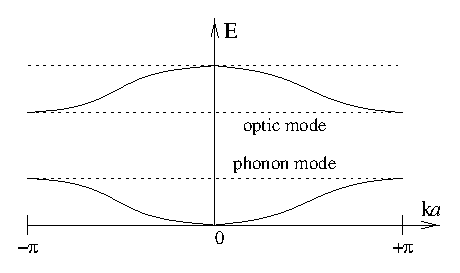
\includegraphics[clip]{1993phy5-1.eps}}
    \end{center}
%

  \SubSubAnswer
    $B%P%s%I%.%c%C%W$O8w3X%b!<%I$H2;6A%b!<%I$H$N4V$N%(%M%k%.!<:9$N(B
    $B:G>.CM$G$"$k!#(B
%
    \[ E_{\rm band gap} = {\rm min}(E^{+} - E^{-}) %
          = \sqrt{(E_A-E_B)^2+16(\gamma-\gamma^{\prime})^2} \]
%
    $B%P%s%I$NI}$O8w3X%b!<%I$H2;6A%b!<%I$H6&$KF1$8$G(B
%
    \[ E_{\rm band width}%
        = \sqrt{(E_A-E_B)^2+16(\gamma+\gamma^{\prime})^2}%
         -\sqrt{(E_A-E_B)^2+16(\gamma-\gamma^{\prime})^2} \]


  \SubSubAnswer
    $BBh(B1Brillouin zone $B$K$O(B$2N$ $B$N>uBV$,$"$k!#(B
    A,B $B86;R$,#1$D$:$DEE;R$r$b$C$F$$$k$H(B$2N$ $B$NEE;R$,$"$k$+$i(B
    $BBh(B1 Brillouin zone $B$N2;6A%b!<%I$,$&$a$D$/$5$l$k!#(B

  \end{subsubanswers}
\end{subanswers}
\end{answer}


\end{document}
